\subsection{Front-end}

% TODO: Mostrar un diagrama de cómo todos los paquetes de bitxenia se utilizan e interactuan entre sí para que el front-end los termine usando. 

Como prueba de la versatilidad de los ecosistemas, y aprovechando la creación de paquetes, se desarrollaron diferentes front-ends para las aplicaciones realizadas.

\paragraph{Astraweb}

Es el principal front-end, y acumula todos los casos de uso creados en una única aplicación web, demostrando la capacidad de utilizar estas herramientas en conjunto, en un entorno web, y de manera intercambiable. Se le permite al usuario escoger el ecosistema al que se desea conectar, pudiendo intercambiar ecosistemas libremente, a forma de comparar y evaluar la funcionalidad desarrollada en este proyecto.

Representa un repositorio de conocimiento, con discusiones en cada articulo, lo que se asemeja a repositorios como Wikipedia. Además, se alojan en las redes descentralizadas evaluadas, tanto en IPFS como en Swarm, accesibles desde el navegador.

\subparagraph{Funcionalidad}

Desde la página principal es posible seleccionar entre tres ecosistemas distintos:

\begin{itemize}
    \item Example Server
    \item IPFS
    \item Blockchain
\end{itemize}

Una vez seleccionado el ecosistema se puede acceder a la barra de búsqueda para buscar el artículo deseado o bien se puede crear un artículo.

En la creación de un artículo \ref{fig:astraweb-create-article}, es posible darle un nombre y una descripción la cual puede ser escrita en Markdown para darle estilo. Una vez dentro de un artículo \ref{fig:astraweb-article-page}, a la derecha se puede acceder al historial de versiones (donde se puede visualizar una versión específica del artículo), editar el artículo (sólo en contenido puede ser modificado) y también al chat del artículo.

Cada artículo posee un chat en tiempo real \ref{fig:astraweb-chat} que actúa como discusión para la mejora o modificación del mismo. Dentro del chat es posible enviar mensajes y responder a mensajes anteriores desde un alias configurado por el usuario. Para mantener la identidad dentro de los chats, se puede ingresar con la misma identificación.

\begin{figure}[H]
    \centering
    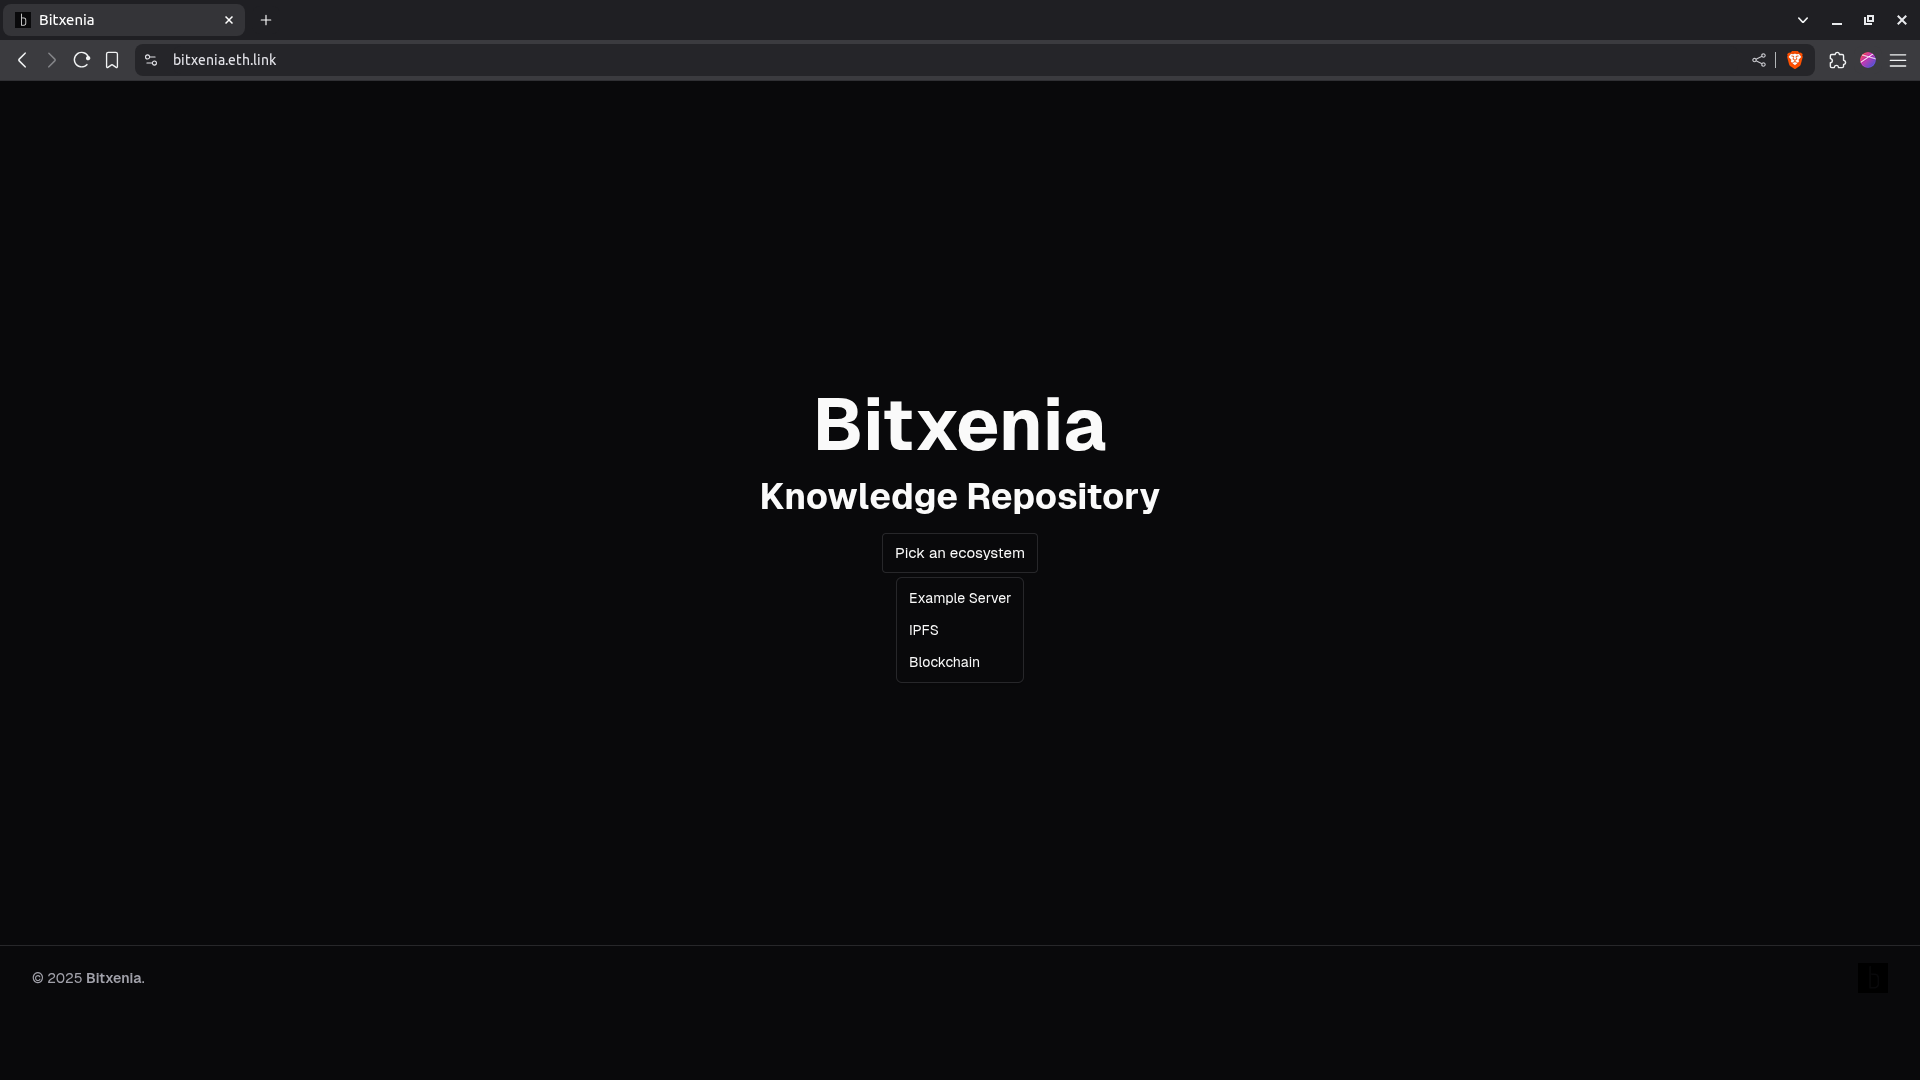
\includegraphics[width=1\linewidth]{img/frontends/astraweb-main-page.png}
    \caption{Página principal de Astraweb}
    \label{fig:astraweb-main-page}
\end{figure}

\begin{figure}[H]
    \centering
    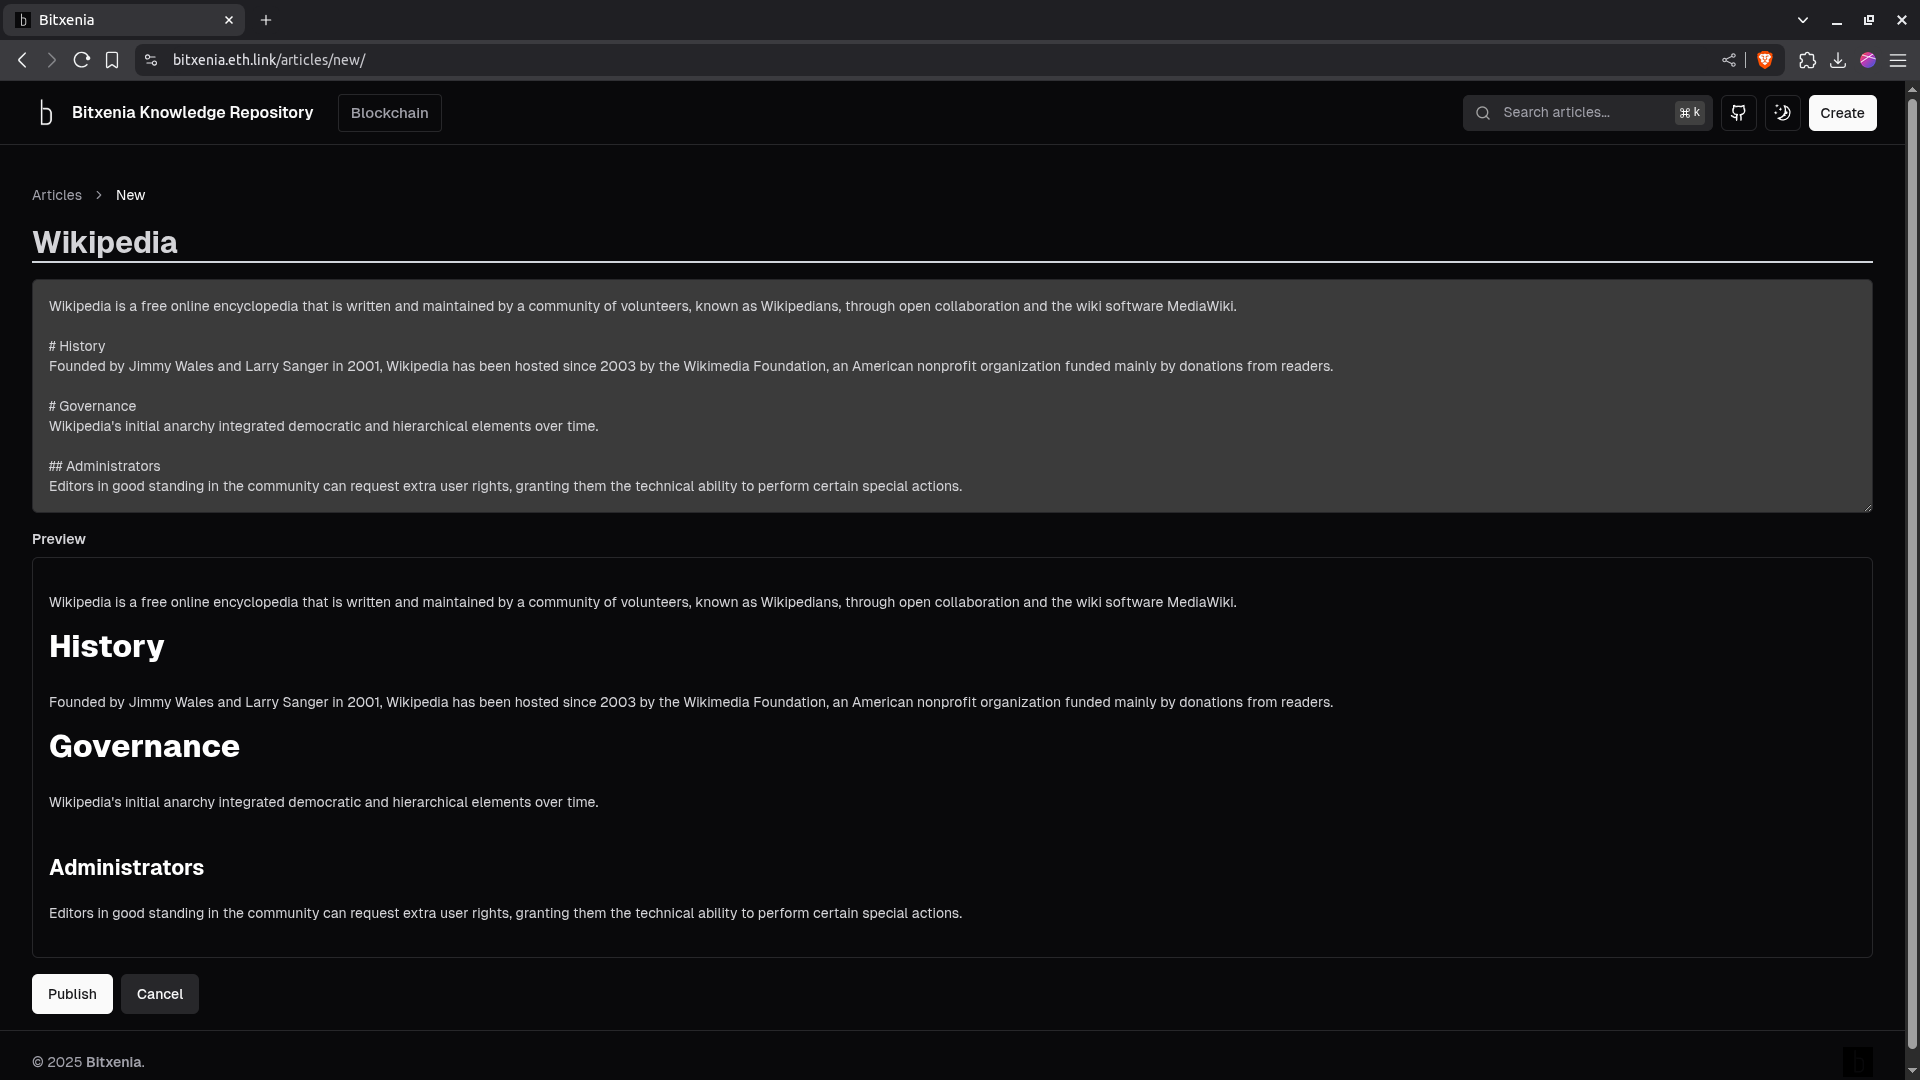
\includegraphics[width=1\linewidth]{img/frontends/create-article.png}
    \caption{Creación de un artículo}
    \label{fig:astraweb-create-article}
\end{figure}

\begin{figure}[H]
    \centering
    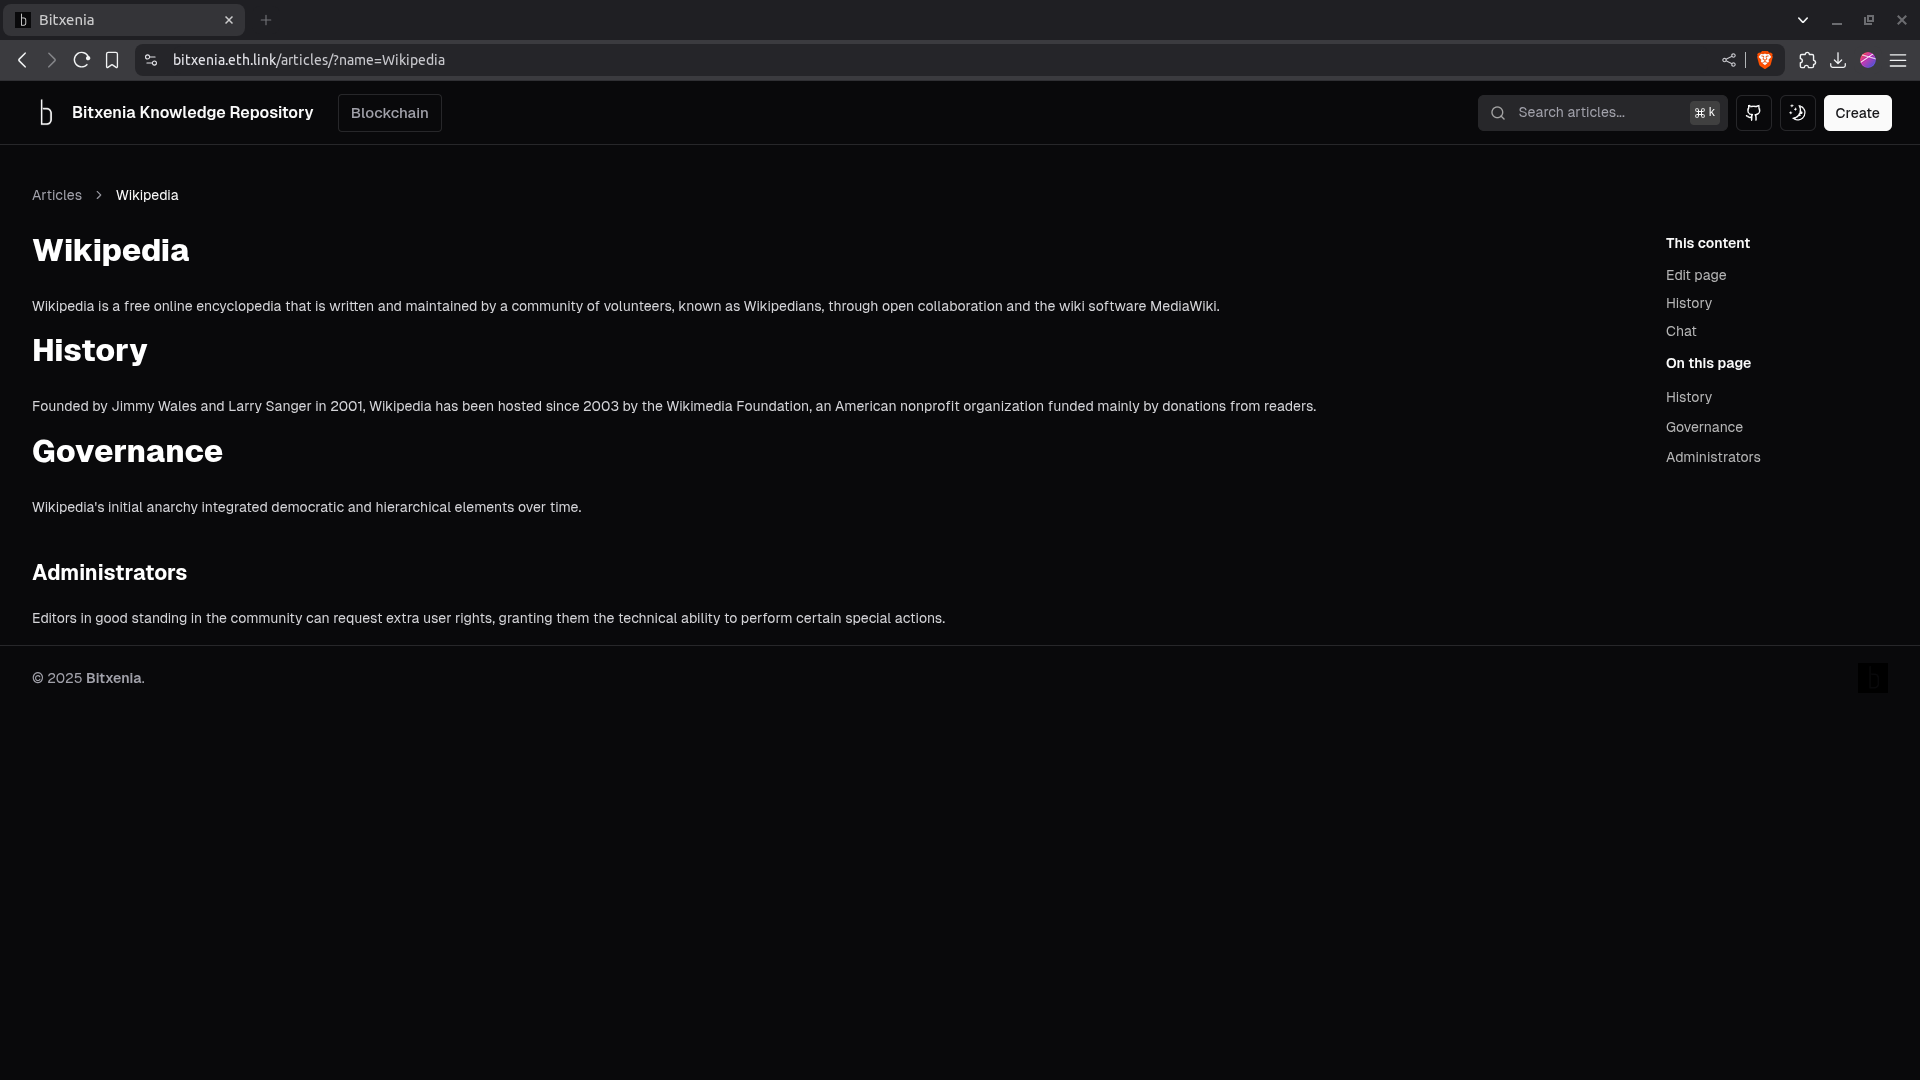
\includegraphics[width=1\linewidth]{img/frontends/article-page.png}
    \caption{Página de un artículo}
    \label{fig:astraweb-article-page}
\end{figure}

\begin{figure}[H]
    \centering
    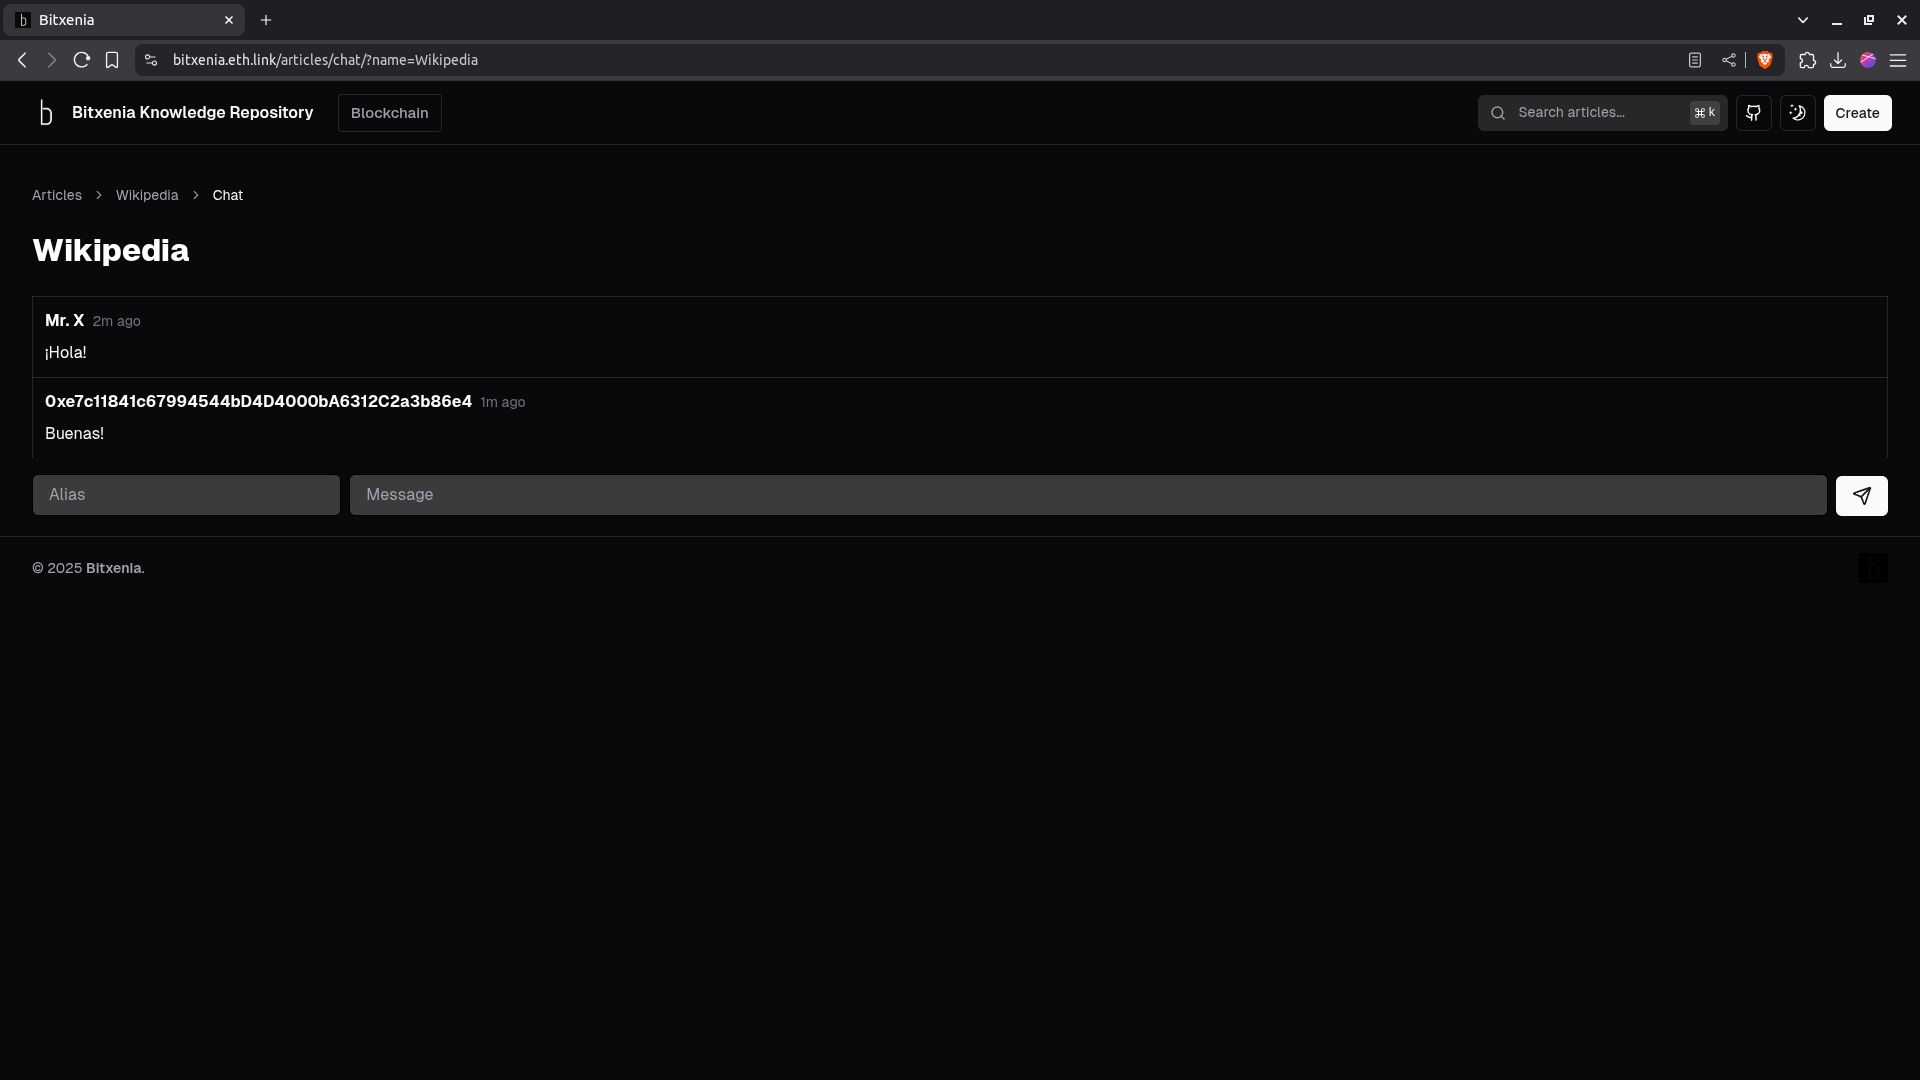
\includegraphics[width=1\linewidth]{img/frontends/astraweb-chat.png}
    \caption{Chat de un artículo}
    \label{fig:astraweb-chat}
\end{figure}

\subparagraph{Tecnología} Se utilizó \texttt{React} \cite{react} y \texttt{Next.js} \cite{next} como \textit{frameworks} para la creación de la aplicación web, basándonos en una plantilla llamada \texttt{rubix-documents} \cite{rubix}. El código fue escrito en \texttt{Typescript}.

\subparagraph{Servidor ejemplo} Se desarrolló una solución centralizada como tercer ecosistema para este frontend, con dos propósitos:
\begin{enumerate}
    \item Paralelizar el desarrollo del front-end y los distintos paquetes de cada ecosistema. Debido a que se definió una interfaz común tanto para el repositorio de conocimiento como para el mensajero en tiempo real, se logró avanzar con el front-end haciendo pruebas manuales con este servidor.
    \item Comparar las implementaciones descentralizadas contra un enfoque centralizado.
    % TODO: esto habría que sacarlo?
\end{enumerate}
El servidor fue creado en \texttt{Node.js} con \texttt{Express.js} como framework para interactuar con \textit{requests} de HTTP.

\subparagraph{Limitaciones} Debido a la falta de un servidor tradicional para ofrecer el contenido, el uso de \textit{Server Components} o componentes de servidor \cite{server-components} no era posible. Esto implicó modificar ampliamente la plantilla utilizada para descartar este tipo de componentes en favor de aquellos que pueden ser compilados y luego utilizados por el cliente sin interacción con un servidor.

\paragraph{Astrawiki CLI}

Front-end de terminal, desarrollado para el caso de uso del repositorio de conocimiento y para el ecosistema de IPFS en específico. Cuenta con todas las funcionalidades del repositorio de conocimiento, como crear, editar y ver artículos, consultar versiones pasadas, e incluso colaborar, lo cual se verá en el apartado de IPFS. Además, cuenta con un contenedor \texttt{Docker} publicado, con el fin de fácilmente iniciar un nodo sin necesitar una instalación de \texttt{Node} y demás dependencias. Funciona como un \texttt{daemon} \cite{daemon}, es decir, se inicia y funciona en segundo plano hasta que se indique lo contrario.

Su propósito es, por un lado demostrar la versatilidad del modelo de paquetes utilizado para crear distintos front-ends. Y por otro lado, el contenedor es útil para el nodo colaborador desarrollado para IPFS visto previamente.

\subparagraph{Arquitectura} Se compone de un cliente, el cuál se inicia con cada comando (\texttt{start}, \texttt{add}, \texttt{get}, \texttt{edit}, \texttt{list}, etc.) y un servidor que se ejecuta por detrás, el cual inicia la instancia del repositorio de conocimiento de IPFS y utiliza su API cuando recibe \texttt{requests HTTP}.

\begin{figure}[H]
    \centering
    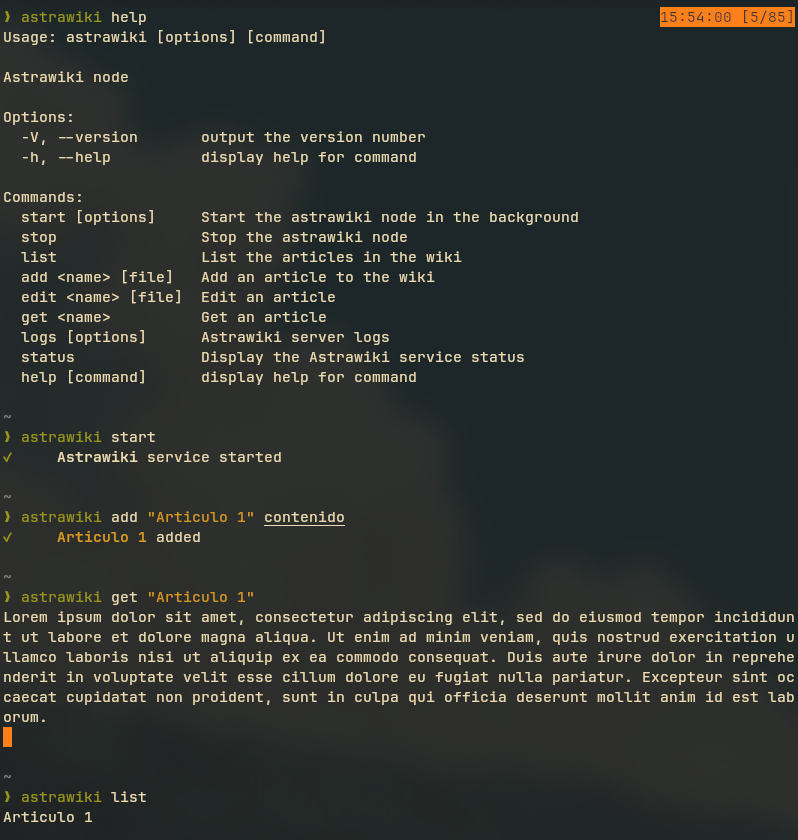
\includegraphics[width=0.7\linewidth]{img/astrawiki-cli.png}
    \caption{Ejemplo de uso de \texttt{astrawiki-cli}}
    \label{fig:astrawiki-cli}
\end{figure}

\paragraph{Astrachat CLI}

Frontend de terminal, desarrollado para el caso de uso de mensajero en tiempo real y para el ecosistema de Blockchain.

\subparagraph{Tecnología}

Se utilizó \texttt{React} \cite{react} y \texttt{Ink} \cite{ink} como \textit{frameworks} para crear la interfaz de este frontend.

\subparagraph{Funcionalidad}

Esta implementación permite crear un chat, unirse a un chat existente, enviar y leer los (últimos) mensajes. No provee de la opción de modificar el alias ni tampoco de responder a otro mensaje.

\begin{figure}[H]
    \centering
    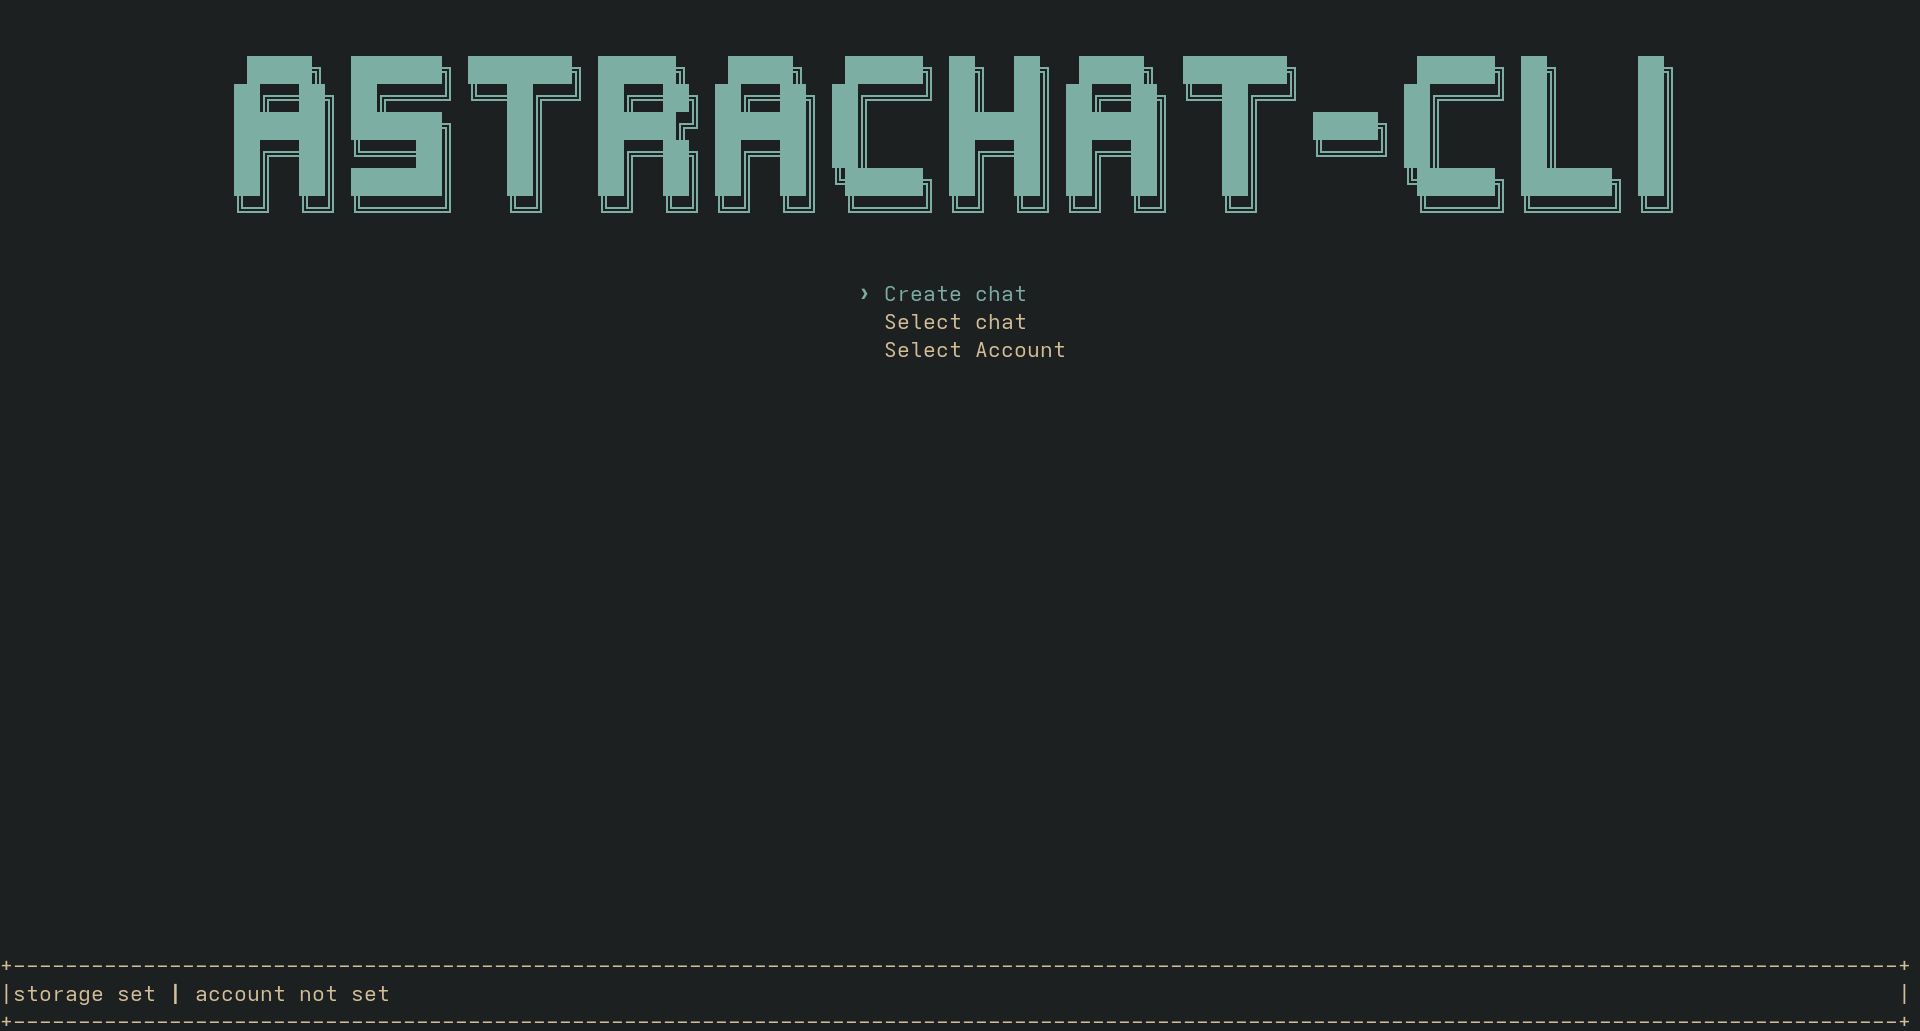
\includegraphics[width=1\linewidth]{img/astrachat-cli-main-page.png}
    \caption{Página principal de \texttt{astrachat-cli}}
    \label{fig:astrachat-cli-main-page}
\end{figure}

\subparagraph{Limitaciones}

Debido a que se ejecuta en la terminal no es posible hacer uso de una wallet como Metamask \cite{metamask} ya que la misma sólo funciona en web. Debido a esto, se \textit{hardcodearon} algunas de las wallets que provee Hardhat \cite{hardhat}.